\documentclass{article}

\usepackage{polski}
\usepackage[utf8]{inputenc}
\usepackage{graphicx}

 \usepackage{geometry} 
\newgeometry{tmargin=1.5cm, bmargin=1.5cm, lmargin=1.5cm, rmargin=1.5cm} 

\begin{document}

\begin{enumerate}
{\Large \bf  \item Scharakteryzuj obszary zastosowań badań nieniszczących w produkcji
przemysłowej.} [Damian H.]

{\Large \bf  \item Scharakteryzuj związki między fizycznymi i psychologicznymi parametrami fali
dźwiękowej.} [Damian H.]

{\Large \bf  \item Omów dwie znane Ci nieniszczące metody badania materiałów oparte o
wykorzystanie fal akustycznych.} [Jakub B.]

 

Wykorzystanie w tym celu fal ultradźwiękowych (wysoka częstotliwość drgań).
np.:

\begin{itemize}
\item Metoda cienia (transmisyjna):

Wymaga użycia dwóch przetworników i transmisji fali od jednego przetwornika do drugiego poprzez badany obszar materiału. Rejestrujemy wtedy natężenie fali przechodzącej przez materiał, a każda nieciągłość powoduje iż w rejestrowanym sygnale powstaje cień. (każda wada materiału powoduje odbicie lub osłabia fale). Nie daje nam jednak informacji gdzie dokładnie (na jakiej głębokości) znajduje się defekt. Nadaje się do badania przedmiotów o grubości maksymalnie 5 cm. 

\item Metoda echa (wykład)


\item Metoda emisji akustycznej 

W badanym elemencie "przykładamy"  zewnętrzną siłę w badanym elemencie (siła ta wytwarza w elemencie naprężenia oraz dyslokacje). Po usunięciu zewnętrznej siły element powraca do swojego stanu początkowego, a co za tym idzie wewnątrz powstają minimalne drgania o wysokiej częstotliwości (na powierzchni mogą powstawać wybrzuszenia). Na powierzchni powinny znajdować się czujniki które będą rejestrować dane zmiany i pozwolą zlokalizować  defekty lub tez nieciągłości materiału. Siłę  zewnętrzną możemy zastąpić nagłą zmiana temperatury lub też ciśnienia. 
( Rys prezentacja 2 slajd ostatni)

\begin{figure}[h!]
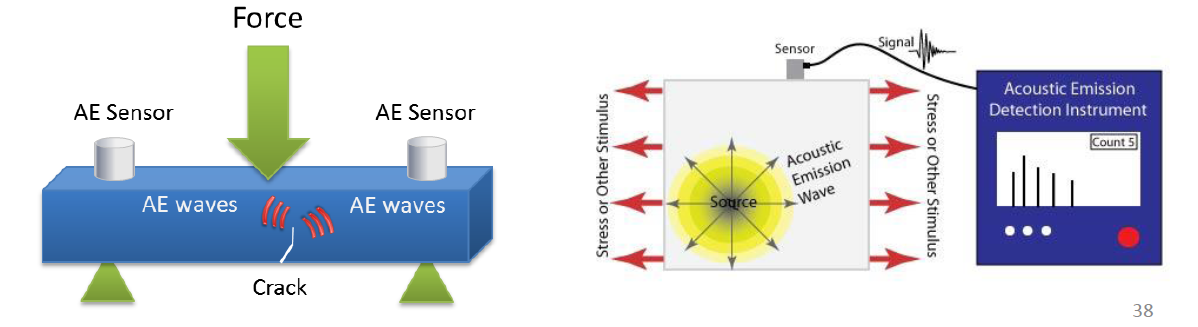
\includegraphics[width=\textwidth]{include/faleakust}
\end{figure}

\end{itemize}




{\Large \bf  \item Jakie znasz metody badań nieniszczących wykorzystujące pola magnetyczne?}  [Jakub B.]
 

W metodzie do badania nieciągłości na powierzchni elementów ferromagnetycznych,tej używa się proszków ferromagnetycznych  oraz pola magnetycznego pochodzącego od magnesu (lub tez elektromagnesu). 

Cząsteczki proszku ustawiają się wzdłuż linii pola magnetycznego, a więc największa ich ilość przypada w miejscu silnej zmiany pola magnetycznego. Pole magnetyczne przyłożone do materiału powoduje modyfikacje pola w obszarze nieciągłości w taki sposób iż tworzy się tam duży gradient pola. Jeżeli materiał jest wolny od wad linie te będą przebiegać bez zmian kierunku , jeśli natomiast w materiale jest wada w tym miejscu linie pola obrazowane przez proszek będą się odchylać. 
Jeżeli na powierzchni są zarysowania to proszek będzie się w nich oraz dookoła ich  silnie gromadzić. Proszki te zazwyczaj są pokolorowane lub tez mogą być fluorescencyjne co ułatwia badanie materiału. 

Metoda jest szybka łatwa oraz nie niszczy materiału ani go nie brudzi.
Wada: tylko dla materiałów ferromagnetycznych oraz konieczność wcześniejszego rozmagnesowania. 


{\bf Metoda wycieku strumienia magnetycznego }


Ponownie sposób badania materiału ferromagnetycznego. W urządzeniu znajduje się głowica z elektromagnesem która wytwarza pole magnetyczne oraz cewka która służy jako czujnik pola. Dodatkowym elementem jest przetwornik który monitoruje położenie głowicy. Całe urządzenie sprzężone jest z komputerem który analizuje prace urządzenia. Jeżeli w materiale znajduję się wada lub są odchyłki w grubościach są one rejestrowane przez sensor a komputer jest w stanie odtworzyć w którym miejscu znajdowała się wada. 








{\Large \bf  \item Scharakteryzuj nieniszczące metody badań oparte o zastosowanie promieniowania
jonizującego.} [Kamil W.]

{\Large \bf  \item Jakie znasz metody nieniszczących badań materiałowych oparte o zastosowanie
pól elektromagnetycznych?} [Zbigniew G.]

{\Large \bf  \item Podstawy fizyczne metody oznaczania składu elementarnego (spektroskopia
optyczna, XRF)} [Kamil S.]

{\Large \bf  \item Mikroskopia elektronowa (transmisyjna i skaningowa)} [Kamil S.]

{\Large \bf  \item Definicje podstawowych jednostek układu SI} [Andrzej W.]

Układ SI definiuje siedem jednostek miary jako podstawowy zbiór z których tworzone są jednostki pochodne. Te podstawowe jednostki i ich fizyczna wielkość to:
\begin{itemize}
\item    metr – długość
\item     kilogram – masa (uwaga: nie gram)
\item     sekunda – czas
\item     amper – prąd elektryczny
\item     kelwin – temperatura
\item     kandela – światłość
\item     mol – liczność materii
\end{itemize}

{\bf Definicje podstawowych jednostek:}

{\small
\begin{tabular}{cccll}
\hline
\hline
nazwa & symbol & wielkość & def. współczesna & def. historyczna \\ 
\hline
\hline
 &&&odległość, jaką pokonuje światło &$\displaystyle\frac{1}{10^7}$ długości mierzonej wzdłuż\\
metr & m & długość &w próżni w czasie 1/299 792 458 s. &  południka paryskiego \\
&&&&od równika do bieguna.\\
\hline
kilogram&	kg&	masa&	masa międzynarodowego wzorca kilograma
&	Masa jednego litra wody.\\
\hline
&&&	czas równy 9 192 631 770 okresom &\\
&&&promieniowania odpowiadającego przejściu \\ 
sekunda&	s&	czas&między dwoma poziomami F = 3 i F = 4&sekunda to 1/(24$\cdot$60$\cdot$60) doby\\
&&& struktury nadsubtelnej stanu podstawowego\\
&&& $^2S_{1/2}$ atomu cezu $^{133}$Cs”\\
 &&&(w spoczynku w temperaturze 0 K)\\
 \hline
	&&& natężenie  prądu elektrycznego,& zdef. elektrochemicznie jako  \\
&&&który płynąc w dwóch równoległych, & prąd potrzebny do wytrącenia\\
&&&prostoliniowych, nieskończenie długich  &  1.118 [mg] srebra na [s] z roztworu\\
amper&	A&	prąd elek.&przewodach,  umieszczonych w próżni& azotanu srebra. W porównaniu\\
&&& w odległości 1 m od siebie, spowodowałby& do obecnej definicji, różnica \\
&&& wzajemne oddziaływanie przewodów&wynosi 0,015\%.\\
&&& na siebie z siłą równą $2\cdot10^{-7}$ N \\
\hline
&&&jeden kelwin to jednostka temperatury&Skala Celsjusza: skala Kelvina \\
&&& równa 1/273,16 temperatury&opiera się na skali Celsjusza,\\
kelwin&	K	&temperatura& termodynamicznej punktu potrójnego wody.”&lecz jest skalą termodynamiczną\\
&&& (woda: 0,00015576 mola $^2$H na jeden mol $^1$H,& (0 K to zero bezwzględne).\\
&&& 0,0003799 mola $^{17}$O na jeden mol $^{16}$O\\
&&& i 0,0020052 mola ${^18}$O na jeden mol $^{16}$O\\
\hline
&&&	liczność materii układu, zawierającego\\
&&& liczbę cząstek równą liczbie atomów& Masa cząsteczkowa \\
&&& zawartych w dokładnie 0,012 kg izotopu&podzielona przez 1 g/mol.\\
mol&	mol&	liczność materii& węgla $^{12}$C. W definicji zakłada się, że \\
&&&węgiel jest w stanie niezwiązanym chemicznie,\\
&&& w spoczynku, a jego atomy nie znajdują\\
&&& się w stanie wzbudzenia.”\\
\hline

&&&	 światłość z jaką świeci w określonym\\
&&& kierunku źródło emitujące promieniowanie\\
kandela&	cd&	światłość& monochromatyczne o częstotliwości&Wcześniejszą jednostką\\
&&& 5,4·1014 Hz i wydajności energetycznej&światłości była świeca.\\
&&& w tym kierunku równej\\
&&& (1/683) [W] na [srad]\\
\hline\hline	
  
\end{tabular}
}


{\Large \bf  \item Podstawowe fakty historyczne związane ze współpracą międzynarodową w
zakresie ustalenia jednolitych jednostek miar.} [Andrzej W.]


{\bf I Generalna Konferencja Miar} z 26 września 1889 r. ustaliła (obowiązującą do 1960 r.) {\bf definicję metra} jako odległości w temperaturze 0$^\circ$C i przy normalnym ciśnieniu atmosferycznym między dwiema głównymi {\bf kreskami na platynowoirydowym wzorcu}, złożonym w Międzynarodowym Biurze Miar w Sèvres pod Paryżem, oraz (nadal obowiązującą) {\bf definicję i wzorzec kilograma}.

{\bf IX Generalna Konferencja Miar} w 1948 r. rozpisała ankietę dotyczącą wprowadzenia nowego układu miar po szeregu krytycznych studiów na temat dotychczasowego (niedoprecyzowanego) układu (w szczególności miano wybrać czwartą jednostkę podstawową, dla pomiaru wielkości elektrycznych, spośród sześciu zaproponowanych). Wprowadziła {\bf (nadal obowiązującą) definicję ampera}, jako jednej z proponowanych w ankiecie jednostek. Ustaliła (obowiązującą do 1979 r., z drobną poprawką) definicję kandeli.

{\bf X Generalna Konferencja Miar} w 1954 r. ustanowiła sześć jednostek podstawowych (metr, kilogram, sekunda, amper, kandela, stopień Kelvina), i przyjęła zasadę spójności układu jednostek podstawowych. Wybrała amper, jako elektryczną jednostkę podstawową. Ustaliła (nadal obowiązującą, z późniejszą poprawką) definicję stopnia Kelvina (nazwa zmieniona w 1967 r.). Wprowadziła definicję jednostki ciśnienia – atmosfery fizycznej.

{\bf XI Generalna Konferencja Miar} w Paryżu w październiku 1960 r. ustanowiła ostatecznie międzynarodowy układ jednostek, wprowadzając dlań {\bf skrót SI} (Système International d'Unités). Zatwierdziła (obowiązującą do 1967 r.) definicję sekundy, używaną obecnie tylko dla celów astronomicznych jako 1/31 556 925,9747 część roku zwrotnikowego 1900 stycznia 0 godzina 12:00, czasu efemeryd. Przyjęła nową (obowiązującą do 1983 r.) definicję metra jako długości równej 1 659 763,73 długości fali promieniowania w próżni odpowiadającego przejściu między poziomami $2$p$^{10}$ a 5d$^5$ atomu $^{86}$Kr. {\bf Oficjalnie wprowadzono przedrostki.}


XIII Generalna Konferencja Miar w październiku 1967 r. wprowadziła nową nazwę jednostki temperatury – kelwin i drobną poprawkę w jej definicji. Przyjęła nową (obecnie obowiązującą) definicję sekundy, opartą na wzorcu odtwarzalnym w warunkach laboratoryjnych. Wprowadziła przeliczenie jednostki ciśnienia atmosfery fizycznej na jednostki SI. Wprowadziła drobną poprawkę w definicji kandeli, uwzględniającą to przeliczenie.

{\bf XIV Generalna Konferencja Miar} w październiku 1971 r. wprowadziła do układu SI, jako jego siódmą jednostkę podstawową, jednostkę ilości (liczności) substancji {\bf mol}, i przyjęła jej (obecnie obowiązującą) definicję. Zatwierdziła nową nazwę jednostki ciśnienia – paskal.

{\bf XVI Generalna Konferencja Miar} w październiku 1979 r. przyjęła {\bf nową (obecnie obowiązującą) definicję kandeli}.

{\bf XVII Generalna Konferencja Miar} w październiku 1983 r. przyjęła (21 X) {\bf nową (obecnie obowiązującą) definicję metra}.

 
 




{\Large \bf  \item Z jakimi metodami fizycznymi zapoznałeś się przy badaniu materiałów węglowo-
grafitowych (SGL-Racibórz)} [Kamil W.]
\end{enumerate}



\end{document}